% -------------------------------------------------------------
% INTRODUCTION
% -------------------------------------------------------------
\section{Project Objectives and Requirements}

\hspace*{1cm}The objective of the HeatItOn project is to develop an automated system that can generate cost-efficient heat production schedules for the district heating network in Heatington. The system aims to replace the current manual planning process by delivering optimized heat-production schedules that meet heat demand, reduce operational costs and ensure efficient use of energy resources. To achieve this, the system must support several key requirements: it must allow users to input relevant source data, manage and select production assets, execute an optimization algorithm that produces feasible and cost-effective schedules, process the resulting output data, and present the results through clear graphical and structured visualizations. The project was developed using a modular software engineering approach, combining .NET C\#, MySQL database for data storage, and an Avalonia-based frontend. Communication between components was handled through API clients and the development process included requirement analysis, system design, implementation  and testing to ensure that each module functioned reliably within the overall system. 

\section{Problem Statement}
\hspace*{1cm}This project addressed the challenge of developing an automated heat production optimization system for HeatItOn, a centralised 
heating utility in the city of Heatington responsible for supplying heat 
to approximately 1600 buildings. The desired outcome was a working 
application capable of automatically generating cost-efficient heat 
production schedules, ensuring that the heat demand of the network was 
met at all times while keeping operational costs as low as possible \cite{projectdata}.

\hspace*{1cm}The system had to account for different types of production units. Some units simply burn fuel to produce heat, meaning their production costs are fixed and predictable. However, other units are also connected to the electricity grid. A gas motor produces electricity as a byproduct which can be sold back to the grid, while an electric boiler consumes electricity which must be purchased. Since electricity prices change every hour, the effective cost of running these units varies constantly, requiring the optimizer to recalculate and compare the costs of all units on an hourly basis in order to always produce the most economical schedule.  

\hspace*{1cm}This required implementing two distinct optimization 
scenarios. The first was a heat-only scenario using three gas boilers 
and one oil boiler. The second was a combined heat and electricity 
scenario using two gas boilers, one gas motor, and one electric boiler. 
Both scenarios also required support for mandatory maintenance periods 
of 30 to 60 hours for designated units, during which the affected unit 
could not participate in the optimization. 

\hspace*{1cm}Prior to this project, all heat production planning at HeatItOn was 
carried out manually. Operators had to select which production 
units to run in each hour based on experience and rough cost estimates. 
This made it particularly difficult to react to changing conditions 
such as fluctuating electricity prices or varying heat demand 
throughout the day. As a result, the process was time-consuming and prone to 
producing inefficient decisions. By automating this process, the aim was to make heat production planning 
more reliable and cost-efficient.




\subsection*{Problem Analysis}

\hspace*{1cm}HeatItOn is a district heating utility in the city of Heatington, responsible for supplying heat to approximately 1,600 buildings via a centralized network. Heat is generated by a combination of traditional heat-only boilers and combined heat and power (CHP) units, which simultaneously produce heat and either generate or consume electricity \cite{lund20144gdh}. 
In a centralized district heating system, hot water is pumped from a central production plant through underground pipes to connected buildings, where it is used for space heating and hot tap water. Once the heat has been extracted, the cooled water flows back to the plant, where it is reheated and recirculated throughout the network.

System will consist of 5 main modules:

\begin{itemize}
    \item Optimizer (OPT)
    \item Data Visualization (DV)
    \item Asset Manager (AM)
    \item Source Data Manager (SDM)
    \item Result Data Manager (RDM)
\end{itemize}

\textbf{Optimizer (OPT):}
Optimizer (OPT): Evaluate all available production units and calculates the most economical heat production schedule, guaranteeing that heat demand across all buildings is met at all times. Each production unit has a fixed cost expressed in DKK per MWh.  The source data for this module is provided in the 2026 Heat Production Optimization – Danfoss Deliveries file.


\textbf{Data Visualization (DV):}
Presents asset, source, and result data in a visual format, enabling users to easily read and analyze the optimization outcomes.

\textbf{Asset Manager (AM):}
Serves as a repository for static system information, providing it available to other system modules. Through the AM, modules can retrieve heating grid information including unit names and graphical representations of the grid.


\begin{figure}[h]
    \centering
    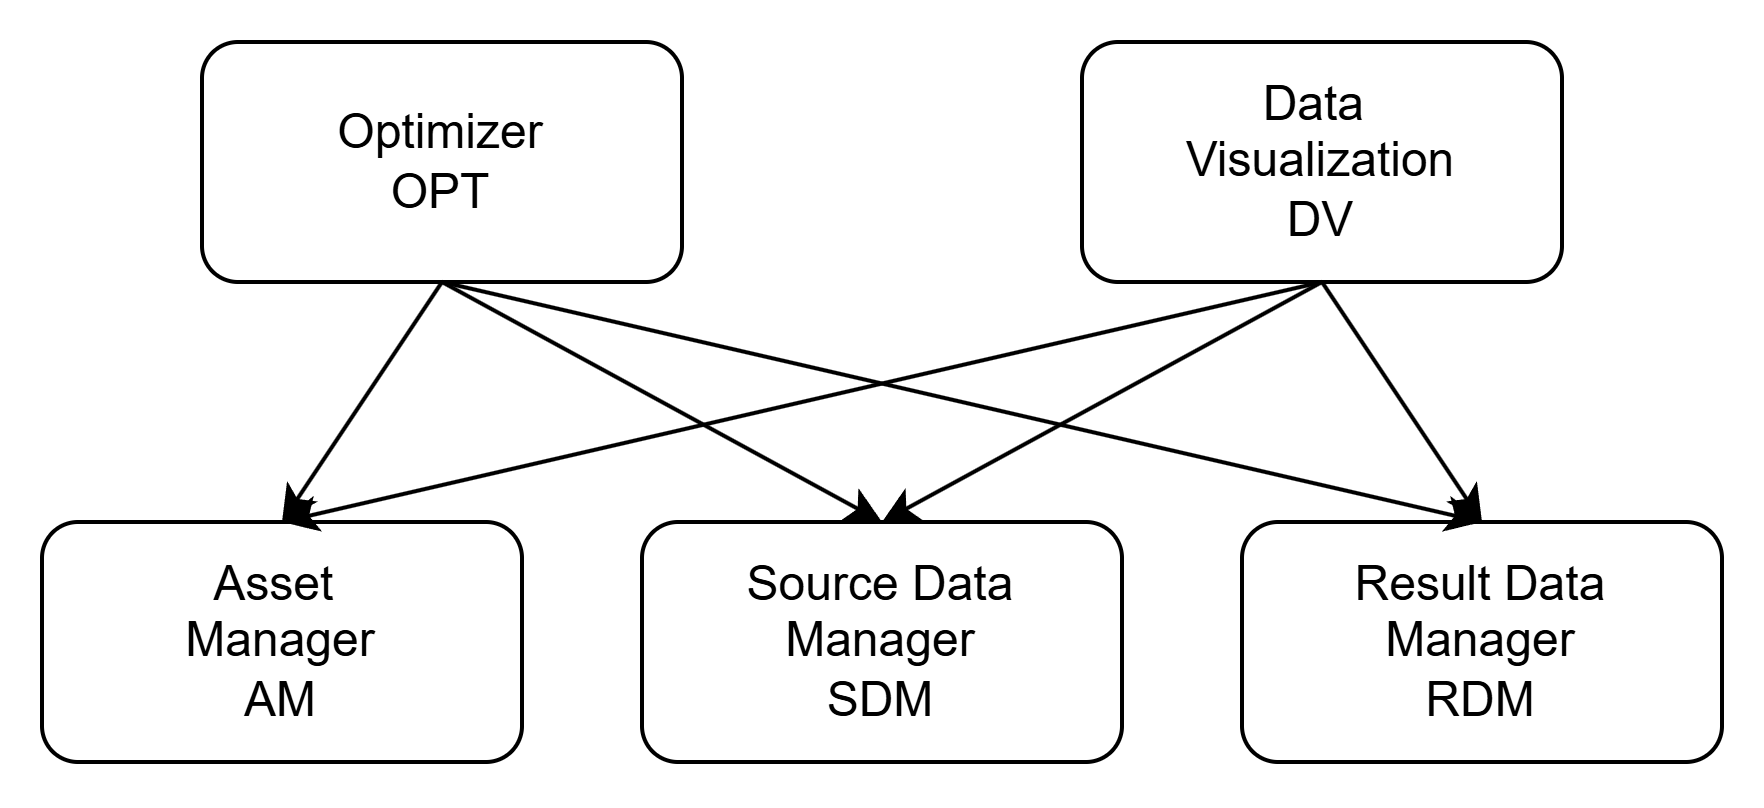
\includegraphics[width=0.8\textwidth]{Images/architecture.png}
    \caption{System Architecture Diagram}
    \label{fig:system-architecture}
\end{figure}

\textbf{Source Data Manager (SDM):}
Serves as a repository for dynamic system information, storing data in local CSV files. The SDM stores and provides two types of data, the amount of heat demanded by the buildings and the current electricity prices, both of which are updated on an hourly basis.

\textbf{Result Data Manager (RDM):}
Scenario 1 operates on a single district heating network with three gas boilers (GB1, GB2, GB3) and one oil boiler (OB1). The gas boilers have lower production costs, while the oil boiler is more expensive and is therefore reserved for peak demand periods. All boilers maintain constant production costs regardless of the hour of operation.
The optimization strategy prioritizes the cheapest gas boiler first, adding output from more expensive units only when needed to meet the total heat demand. One of the gas boilers must also undergo a scheduled maintenance period of between 30 and 60 hours, during which it is taken offline and produces 0 MW.



\subsection*{Scenarios}

\subsubsection*{Scenario 1 (Heat only)}

\hspace*{1cm}Scenario 1 uses a single district heating network with three gas boilers (GB1, GB2, GB3) and one oil boiler (OB1). The gas boilers are cheaper, while the oil boiler has higher production costs and is mainly used in peak demand periods. All boilers have constant production costs that do not depend on the hour of operation. Strategy for scenario one is to run the cheapest gas boiler first and then add production from the more expensive boilers if needed to meet the heat demand. There should also be chosen a period of 30 to 60 hours when one of the gas boilers will be down due to maintenance.

\subsubsection*{Scenario 2 (Heat and electricity)}

\hspace*{1cm}Scenario 2 operates on a network with two gas boilers (GB1, GB3), one gas motor (GM1), and one electric boiler (EB1). The gas motor produces electricity that can be sold on the market, while the electric boiler consumes electricity that must be purchased.
When electricity prices are high, the gas motor is prioritized, as selling electricity generates additional income. When prices are low, the electric boiler becomes the preferred unit, as buying electricity is cheaper. Unit selection is determined each hour by calculating and comparing the net production cost for each unit.


The project is based on data delivered by Danfoss, including:

\begin{itemize}
    \item Graphical representation of the district heating network
    \item Configuration parameters for each production unit (image, produced heat, produced/consumed electricity, primary energy consumption, production costs, CO2 emissions)
    \item Heat demand and electricity prices for a 14-day winter period with 1-hour resolution
    \item Heat demand and electricity prices for a 14-day summer period with 1-hour resolution
\end{itemize}

\medskip

\hspace*{1cm}If there is time left,  project can be extended by usage of other visualization libraries, storing data in a database, enabling or disabling units directly from the UI, running alternative configurations in Scenario 2, and implementing APIs and an API client for reading electricity prices from Energinet.dk.

\section{Functional Requirements}

\hspace*{1cm}The following tables outline the formal functional requirements for the system, translated into standardized system-level behaviors. The requirements are divided into three tables: one for each of the two operational scenarios, and a third covering general app navigation and UI requirements.

\vspace{0.5cm}

% --- TABLE 1: Scenario 1 ---
\renewcommand{\arraystretch}{1.5}
\begin{longtable}{|p{1.5cm}|p{2.4cm}|p{6.7cm}|p{1.4cm}|p{2cm}|}
\caption{Functional Requirements: Scenario 1}
\label{tab:fr_scenario1} \\
\hline
\textbf{ID} & \textbf{Related US} & \textbf{Requirement Description} & \textbf{Priority} & \textbf{Notes} \\
\hline
\endfirsthead

\multicolumn{5}{c}{{\tablename\ \thetable{}: Functional Requirements: Scenario 1}} \\
\hline
\textbf{ID} & \textbf{Related US} & \textbf{Requirement Description} & \textbf{Priority} & \textbf{Notes} \\
\hline
\endhead

\hline \multicolumn{5}{|r|}{{Continued on next page}} \\ \hline
\endfoot

\hline
\endlastfoot

FR-001 & HEAT - 78/79 & The system shall allow the user to input data. & High & SDM\&RDM \\
\hline
FR-002 & HEAT - 78/79 & The system shall allow the user to retrieve input data. & High & SDM\&RDM \\
\hline
FR-003 & HEAT - 79 & The system shall allow the user to output data. & High & Database integration \\
\hline
FR-004 & HEAT - 79 & The system shall allow the user to upload assets from a CSV file. & High & Asset Manager \\
\hline
FR-005 & HEAT - 82 & The system shall allow the user to add an asset. & High & Asset Manager \\
\hline
FR-006 & HEAT - 82 & The system shall allow the user to edit assets. & High & Boiler definitions \\
\hline
FR-007 & HEAT - 188 & The system shall allow the user to restrict the maximum heat output of each unit as follows: GB1 to 3.0 MW, GB2 to 2.0 MW, GB3 to 4.0 MW, and OB1 to 6.0 MW. & Critical & Capacity constraints \\
\hline
FR-008 & HEAT - 146 & The system shall allow the user to schedule the cheapest boilers first to fulfill the district’s heat demand. & Critical & Cost-based dispatch \\
\hline
FR-009 & HEAT - 146 & The system shall prioritize boilers in the following strict order based on production costs: GB1 (510 DKK), GB2 (540 DKK), GB3 (580 DKK), and OB1 (690 DKK). & Critical & Dispatch order \\
\hline
FR-010 & HEAT - 188 & The system shall allow the user to use the more expensive oil boiler (OB1) only to supplement heat during peak demand periods when the gas boilers cannot fulfill the total demand. & High & Peak demand handling \\
\hline
FR-011 & HEAT - 188 & The system shall allow the user to optimize units separately for both a winter period and a summer period. & High & Seasonal optimization \\
\hline
FR-012 & HEAT - 146 & The system shall remove a designated gas boiler from the available pool of units during its scheduled maintenance period, ensuring it produces 0 MW. & Medium & Maintenance logic \\
\hline
FR-013 & HEAT - 146 & The system shall validate that the user’s selected maintenance duration is a minimum of 30 hours and a maximum of 60 hours. & Medium & Maintenance validation \\
\hline
FR-014 & HEAT - 147/148 & The system shall display a chart or graph that visually compares the total heat demand against the individual heat output contributions of GB1, GB2, GB3, and OB1 over time. & High & Result graphing \\
\hline
FR-015 & HEAT - 188 & The system shall allow the user to choose an obligatory maintenance period for one unit in both the summer and winter periods. & Medium & Maintenance scheduling \\
\end{longtable}


% --- TABLE 2: Scenario 2 ---
\begin{longtable}{|p{1.5cm}|p{2.4cm}|p{6.7cm}|p{1.4cm}|p{2cm}|}
\caption{Functional Requirements: Scenario 2}
\label{tab:fr_scenario2} \\
\hline
\textbf{ID} & \textbf{Related US} & \textbf{Requirement Description} & \textbf{Priority} & \textbf{Notes} \\
\hline
\endfirsthead

\multicolumn{5}{c}{{\tablename\ \thetable{}: Functional Requirements: Scenario 2}} \\
\hline
\textbf{ID} & \textbf{Related US} & \textbf{Requirement Description} & \textbf{Priority} & \textbf{Notes} \\
\hline
\endhead

\hline \multicolumn{5}{|r|}{{Continued on next page}} \\ \hline
\endfoot

\hline
\endlastfoot

FR-016 & HEAT - 40/91/92 & The system shall allow the user to retrieve hourly electricity prices data from the database. & High & SDM\&RDM \\
\hline
FR-017 & HEAT - 91/92 & The system shall allow the user to retrieve hourly heat demand data from the database. & High & Market data retrieval \\
\hline
FR-018 & HEAT - 79/277 & The system shall allow the user to upload assets from a CSV file. & High & Unit registration \\
\hline
FR-019 & HEAT - 146 & The system shall allow the user to limit the maximum heat output of each unit: GB1 to 3.0 MW, GB3 to 4.0 MW, GM1 to 5.3 MW, and EB1 to 6.0 MW. & High & Heat capacity constraints \\
\hline
FR-020 & HEAT - 146 & The system shall allow the user to account for electricity production and consumption capacities, specifically noting that GM1 produces up to 3.9 MW of electricity, while EB1 consumes up to 6.0 MW (-6.0 MW). & High & Electricity constraints \\
\hline
FR-021 & HEAT - 188/203 & The system shall allow the user to calculate the net production costs for the electricity-producing/consuming units based on fluctuating electricity prices. & High & Dynamic net cost calculation \\
\hline
FR-022 & HEAT - 188 & The system shall prioritize running the gas motor (GM1) during periods of high electricity prices. & Critical & High-price optimization logic \\
\hline
FR-023 & HEAT - 188 & The system shall prioritize running the electric boiler (EB1) during periods of low electricity prices. & Critical & Low-price optimization logic \\
\hline
FR-024 & HEAT - 188 & The system shall actively prevent the gas motor (GM1) from running during summer periods with negative electricity prices (to avoid paying for produced electricity). & Critical & OPT \\
\hline
FR-025 & HEAT - 188 & The system shall recognize the electric boiler as an extra income source during negative price hours. & High & Negative price handling \\
\hline
FR-026 & HEAT - 146 & The system shall completely remove either GB1 or GM1 from the optimization calculations during its scheduled maintenance period. & High & Maintenance logic \\
\hline
FR-027 & HEAT - 146 & The system shall allow the user to select an obligatory maintenance period for either GB1 or GM1, and enforce a duration between 30 and 60 hours. & Medium & Maintenance scheduling \\
\hline
FR-028 & HEAT - 146 & The system shall display a graph comparing the total heat demand against the individual heat output contributions of GB1, GB3, GM1, and EB1 over time. & Medium & Result graphing \\
\end{longtable}


% --- TABLE 3: General App Navigation and UI ---
\begin{longtable}{|p{1.5cm}|p{2.4cm}|p{6.7cm}|p{1.4cm}|p{2cm}|}
\caption{Functional Requirements: General App Navigation \& UI.}
\label{tab:fr_general} \\
\hline
\textbf{ID} & \textbf{Related US} & \textbf{Requirement Description} & \textbf{Priority} & \textbf{Notes} \\
\hline
\endfirsthead

\multicolumn{5}{c}{{\tablename\ \thetable{} -- continued from previous page}} \\
\hline
\textbf{ID} & \textbf{Related US} & \textbf{Requirement Description} & \textbf{Priority} & \textbf{Notes} \\
\hline
\endhead

\hline \multicolumn{5}{|r|}{{Continued on next page}} \\ \hline
\endfoot

\hline
\endlastfoot

FR-029 & HEAT - 149 & Upon launch, the system shall display a home screen allowing the user to explicitly select between Scenario 1 and Scenario 2. & High & Startup Page \\
\hline
FR-030 & HEAT - 149 & The system shall allow the user to easily navigate between scenarios. & High & Scenario navigation \\
\hline
FR-031 & HEAT - 91/92/233 & The system shall allow the user to use a database system to save and retrieve data. & High & Database storage \\
\hline
FR-032 & HEAT - 84/85 & The system shall allow the user to dynamically activate or deactivate individual heating units from being considered in the optimizer’s calculations. & High & Dynamic unit toggling \\
\hline
FR-033 & HEAT - 84 & The system shall allow the user to run a custom scenario with configurations set by the user. & High & Custom scenario configuration \\
\hline
FR-034 & HEAT - 147/188 & The system shall provide results of different configured scenarios for result comparison. & High & Comparison metrics \\
\end{longtable}

\newpage
\section{Non-Functional Requirements}

\hspace*{1cm}The following table details the non-functional requirements (NFRs), which define the system's quality attributes, performance standards, and operational constraints.

\vspace{0.5cm}

% --- TABLE 4: Non-Functional Requirements ---
\begin{longtable}{|p{2cm}|p{8cm}|p{4cm}|}
\caption{Non-Functional Requirements detailing system quality attributes.}
\label{tab:non_functional_requirements} \\
\hline
\textbf{ID} & \textbf{Requirement Description} & \textbf{Notes} \\
\hline
\endfirsthead

\multicolumn{3}{c}{{\tablename\ \thetable{}: Non-Functional Requirements detailing system quality attributes.}} \\
\hline
\textbf{ID} & \textbf{Requirement Description} & \textbf{Notes} \\
\hline
\endhead

\hline \multicolumn{3}{|r|}{{Continued on next page}} \\ \hline
\endfoot

\hline
\endlastfoot

NFR-001 & The system shall complete all optimization calculations within 3 seconds of the user clicking 'Optimize'. & Optimization speed \\
\hline
NFR-002 & The system shall completely render the resulting graphs within 3 seconds of the user clicking 'Optimize'. & Processing speed \\
\hline
NFR-003 & The system shall efficiently load, process, and aggregate a full month of hourly data (approximately 720-744 data points) without UI freezing or lag. & Data volume handling \\
\hline
NFR-004 & The system shall be fully cross-platform compatible, executing reliably on Windows, macOS, and Linux operating systems. & Cross-platform compatibility \\
\hline
NFR-005 & The system shall present the entire user interface, including all menus, labels, and error messages, in English. & UI Language \\
\hline
NFR-006 & The system shall calculate and display all financial values, production costs, and revenues strictly using Danish Kroner (DKK). & Currency localization \\
\hline
NFR-007 & The system shall generate a highly readable visualization for a month of data, formatting the daily boiler usage as a stacked chart (matching the total heat demand on the Y-axis, and days of the month on the X-axis) alongside a daily cost graph. & Visualization clarity \\
\hline
NFR-008 & The system shall not crash if user loses their internet connection. & System stability \\
\hline
NFR-009 & The system shall handle API failures by displaying a clear, understandable error feedback message or popup to the user. & Exception handling \\
\end{longtable}

\section{System Requirements}
\hspace*{1cm}The system is split into three parts: Front End, Back End and the Database. Both the Backend and the Database are run in a Linux Docker container. The Frontend is run locally on the user's machine. For a machine to run the project they need the following:

\subsection*{Software Specifications}
\begin{description}
    \item[Entire project:] .NET 9.0
    \item[Backend:] Docker Desktop (latest version)
    \item[Database:] Docker Desktop with MySql Image (shall be installed automatically if missing)
    \item[Frontend:] Required NuGet packages (all must be compatible with .NET 9.0):
    \begin{itemize}
        \item Avalonia.UI
    \end{itemize}
\end{description}
